\documentclass{scrreprt}
\usepackage{scrlayer-scrpage}

% Umlaute und Font-Encoding
\usepackage[T1]{fontenc}
\usepackage[utf8]{inputenc}

% Deutsch
\usepackage[ngerman]{babel}

% Das muss fucking nochmal GEIL aussehen!
% \usepackage{microtype} - Erst im Final actimelisieren

% Mathe
\usepackage{amsmath}

% Coole Links im PDF
\usepackage[hidelinks]{hyperref}

% Aliase zum abdrucken von Shell-CMDs
\newcommand{\shellcmd}[1]{\texttt{\$ #1}\\}
\newcommand{\shellout}[1]{\texttt{#1}\\}

% Alias für Aufgabenname
\newcommand{\task}[1]{Kreis-Code}


\ihead{\task} \ohead{Laurenz Grote, Teilnahme 6745 (Team 00001)}
\renewcommand{\chapterpagestyle}{scrheadings}
\pagestyle{scrheadings}

\begin{document}

	\titlehead{Teilnahme 6745 (Team 00001) \hfill Laurenz Grote}
	\title{\task}
	\subtitle{Aufgabe 3}
	\author{Laurenz Friedrich Grote}
	\date{}
	\maketitle
	\tableofcontents
	
	\vspace {2em}
	Meine Umsetzung für "`\task"' erfolgte unter Ubuntu mit Java (OpenJDK 1.8). Ich habe ihnen den Programmcode sowie eine ausführbare .jar-Datei beigelegt.
	\pagebreak
	% ----------------------------------------------------------------------------
	\chapter{Erkennung von Grafiken}
		\section{Lösungsidee}
Um möglichst effizient Kreismittelpunkte zu bestimmen, mache ich mir zunächst folgende Eigenschaft von Kreisen zunutze: Am Mittelpunkt eines Kreises ist der Abstand (Radius) zu der äußeren Umrandung des Kreises in jede Richtung gleich.

In einem Bild lassen sich solche Punkte finden, indem man von jedem schwarzen Bildpunkt misst, wie weit man sich auf dem Bild in vertikale wie horizontale Richtung "`bewegen"' kann, ohne auf ein weißes Feld zu stoßen. Wenn dieser Abstand nach rechts, links, oben und unten gleich groß ist, genügt der Punkt der erstgenannten Eigenschaft von Kreisen. 

Von einem Vergleich des Abstandes in andere Richtungen (wie z.B. in diagonale Richtung) sollte man bei einem Bild aus Pixeln absehen, da bei der Speicherung eines Kreises als Bitmap aus quadratischen Pixeln diagonale Messungen oder gar Messungen unter beliebigem Winkel ungenaue Ergebnisse liefern. Zwar sind solche Messungen prinzipiell möglich, liefern aber anders als rein vertikale oder horizontale Messungen kein ganzzahligen Ergebnisse, da eine Pixeldiagonale \(\sqrt{2}\) Pixelseiten lang ist.
\footnote{: \( \vert \begin{pmatrix}1\\1\end{pmatrix} \vert = \sqrt{2}\)}

\begin{figure}[!ht]
	\centering	
	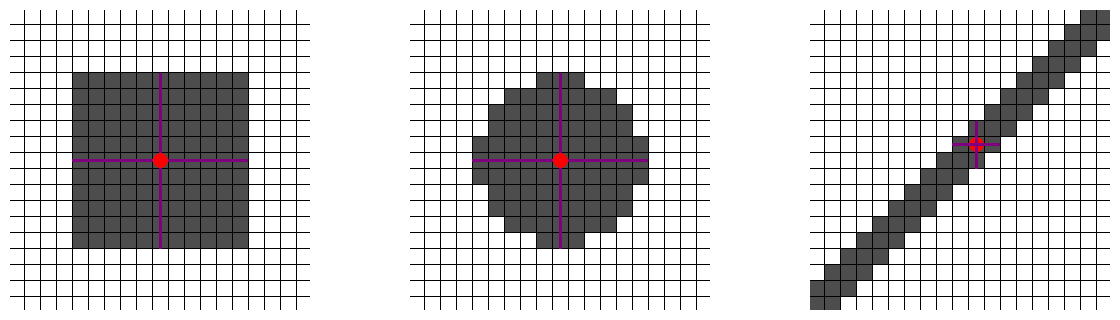
\includegraphics[width=0.8\textwidth]{durchmesservergleich}
	\caption{Versch. Formen mit eingezeichnetem Mittelpunkt (erstes Kriterium)}
\end{figure}

Da diese Eigenschaft jedoch auch auf Punkte in Quadraten und anderen unregelmäßigen Formen zutrifft (s. Grafik), muss für eine zuverlässige Erkennung eine zweite Eigenschaft von Kreisen genutzt werden: Bei bekanntem Durchmesser kann die Fläche eines Kreises mit der Kreisformel\footnote{: \(\frac{\pi d^2}{4}\)} bestimmt werden. Diese Soll-Fläche kann mit der tatsächlichen Fläche verglichen werden. Sollte das Delta zwischen diesen beiden Flächengrößen nahe 0 sein, handelt es sich mit sehr großer Wahrscheinlichkeit um einen Kreismittelpunkt.

Daher nehme ich an, dass jeder Punkt, auf den beide Bedingungen zustimmen, ein Kreismittelpunkt ist. Allerdings gibt es aufgrund von Kompressionsartefakten o.ä. manchmal mehrere Punkte, auf die die Bedingungen zutreffen. Damit der Mittelpunkt eindeutig festgestellt wird, vergebe ich bei der Flood-Fill ID's für jede Zusammenhangskomponente. Daher kann ich für Pixel, für die schon eine ID vergeben wurde, die Suche abbrechen. Schließlich wurde entweder schon ein Mittelpunkt gefunden oder es hat sich herausgestellt, dass es sich nicht um einen Kreis handelt.

\begin{wrapfigure}{r}{0.35\textwidth}
  \centering
  \begin{tikzpicture}[scale=0.3]
\fill[black!90!white] (0,0) circle [radius=1.5];
\fill[black!90!white, even odd rule] (0,0) circle[radius=2.5] circle[radius=3.5];
\fill[black!60!white, even odd rule] (0,0) circle[radius=4.5] circle[radius=5.5];

\foreach \angle in {0, 22.5, 45, 67.590, 90, 112.5, 135, 157.5, 180, 202.5, 225, 247.5, 270, 292.5, 315, 337.5} 
	\draw[thick] (\angle:4.5) -- (\angle:5.5);

\fill[red] (0,0) circle[radius=0.2];

\draw[color=blue!60!violet, thick] (-1.5,1.4) -- ++(0, 0.2) -- ++(1.5, 0) +(0, 0.4)node[black]{\tiny{\(3u\)}}+(0, 0) -- ++(1.5, 0) -- ++(0, -0.2);

\draw[color=blue!60!violet, thick] (0,0) -- (0,-6.7) -- +(-1.5, 0) -- (-1.5,0);
\draw[color=blue!60!violet, thick] (0,0) -- (0,-8) -- +(-2.5, 0) -- (-2.5,0);
\draw[color=blue!60!violet, thick] (0,0) -- (0,-9.3) -- +(-3, 0) -- (-3,0);

\draw (-0.75, -6) node{\tiny{\(\frac{3}{2}u\)}};
\draw (-1.25, -7.4) node{\tiny{\(\frac{5}{2}u\)}};
\draw (-1.25, -8.7) node{\tiny{\(\frac{3}{1}u\)}};
\end{tikzpicture}
  \caption{Größenverhältnisse}
\end{wrapfigure}
Danach gilt es noch zu bestimmen, ob es sich bei dem Kreis um einen Mittelpunkt eines \task{}s handelt, schließlich sollen sonstige Kreise im Bild nicht ausgegeben werden. Hierzu können wir uns die Proportionen eines \task{}s zu nutze machen:

Der Durchmesser ist als \(3u\) definiert, jeder Kreisring und die Zwischenräume haben eine Breite von \(1u\). Daraus folgt, dass wenn man den Mittelpunkt in eine beliebige Richtung um \(3u\) verschiebt, der neue Punkt im mittleren Kreisring liegen muss.

Um nun das Vorhandensein des mittleren Ringes zu überprüfen, nehmen wir vier Punktproben vor. Wir verschieben den Mittelpunkt in alle Himmelsrichtugen um \(u\). Dort vergleichen wir die Länge der entsprechenden linearen Zusammenhangskomponente mit dem Soll \(1u\). Weitere Punktproben sind prinzipiell möglich, jedoch würden diese die Laufzeit erhöhen. \textbf{Ggfs. weitere Flood-Fill auf Fläche des Kreisringes hinzufügen!}

Die Wahrscheinlichkeit eines Erkennungsfehlers ist nach dem Durchmesservergleich, dem Flächenvergleich und den vier Punktproben sehr gering. Im Beispielbild, dass ich um einen Kreis, der kein \task ist ergänzt habe,liegt die Erkennungsrate bei 100\%.

\pagebreak
\section{Umsetzung}
In meiner Implementierung muss das Delta zwischen der Ist- und Soll-Fläche kleiner als 5\% sein.

Zunächst implementierte ich mithilfe von ImageIO eine Bildeinleseprozedur. Da ImageIO nur RGB-JP(E)Gs, PNGs, BMPs und GIFs einlesen kann, habe ich einen Wrapper für ImageMagick\footnote{\url{http://www.imagemagick.org/}, GPLv3-kompatible freie Lizenz. Enthalten in den Repositories der gängigen Linux-Distributionen, Binarys für weitere Betriebssysteme auf der Entwicklerseite.} geschrieben. Wenn dieser über die entsprechende Checkbox in der GUI zugeschaltet wird, können alle gängigen Bildformate gelesen werden. Nachteil ist eine deutlich längere Einlesezeit. Außerdem muss ImageMagick lokal installiert sein und mit dem Befehl \texttt{convert} aufrufbar sein.\footnote{Getestet unter Arch Linux und Ubuntu Linux 16.10. Weitere Betriebssysteme werden vermutlich auch unterstützt.}

Zunächst überlegte ich mir eine möglichst effiziente Datenstruktur für Grafiken, da die Interaktion über ImageIO mit Bitmaps nicht sonderlich effizient ist. Da für die Erkennung von Kreisen in einer Grafik genaue Informationen über die Farbe eines Bildpunktes nicht relevant sind, kann das Bild beim Einlesevorgang in ein boolesches 2D-Array überführt werden: In diesem Array, das die gleiche Größe wie das eingelesene Bild besitzt, sind die Bildpunkte als True gespeichert, die Teil eines \task{}s sein könnten. In der in Teilaufgabe 1 gegebenen Schwarz-Weiß-Grafik ist diese Einstufung noch simpel: Schwarze Bildpunkte können Teil eines \task{}s sein, sonstige nicht.

Um in diesem Array die Punkte zu bestimmen, deren Kreisradien sich in alle vier Richtungen gleichen, bestimme ich zunächst die Länge von aufeinanderfolgenden Streifen aus möglichen \task{}-Feldern. Diese nenne ich nun lineare Zusammenhängigkeitskomponenten. In seperaten Arrays für horizontale und vertikale Streifen speichere ich für jedes Feld die gesamte Länge seiner linearen Zusammenhängigkeitskomponente. \textbf{Zeichnung?} 
Für ein mögliches \task{}-Feld liegt die Länge für horizontale Zusmmenhängikeitskomponenten in \(1 \le l \le width\), für vertikale entsprechend in \(1 \le l \le height\). Allen Feldern, die kein Teil einer Zusmmenhängikeitskomponente sind, haben in den Arrays einen Wert von \(0\). 

Die erste Eigenschaft aus der Aufgabenstellung lässt sich mit dieser Information nun dahingehend vereinfacht werden, dass sich überlappende Mittelpunkte gleich langer Zusammenhängigkeitskomponenten gesucht wird. Dann ist die Eigenschaft gegeben, da in alle Richtungen die Länge gleich ist.

Dafür bestimme ich zunächst alle Mittelpunkte horizontaler linearer Zusammenhängigkeitskomponenten. Dies geschieht, indem ich mit einer linearen Suche über das ganze Bild alle Koordinaten bestimme, deren Zusammenhängigkeitskomponentenlänge größer null ist und der kein Feld vorausgeht, dass Teil einer Zusammenhängigkeitskomponente ist. Feldern am linken Rand gehen grundsätzlich keine Zusammenhängigkeitskomponentenfelder voraus, d. h. dass Komponenten sich meiner Definition nach nicht über Zeilengrenzen hinweg erstrecken. Diese Funktion liefert erst einmal Anfangsstellen von horizontalen Zusammenhängigkeitskomponenten. Wenn ich auf diese Anfangsstelle allerdings nun die Hälfte der Länge der Komponente hinzuaddiere, erhalte ich die x-Koordinate des Mittelpunktes der Zusammenhängigkeitskomponente. Die y-Koordinate ist für eine \textit{horizontale} Komponente durchgehend gleich und daher aus der linearen Suche gegeben.

An dieser Stelle lese ich nun die Länge der vertikalen linearen Zusammenhängigkeitskomponente aus. Wenn die Differenz zwischen dieser und der Länge der horizontalen Komponente 0 oder 1 ist, werte ich die Längen der Komponenten als gleich. Ein Fehler von 1 kann ich durch Rundungsfehler bei ganzzahligen Divisionen entstehen.

Zuletzt überprüfe ich noch, ob der Mittelpunkt der vertikalen Kompontenten auf dem Schnittpunkt der beiden Komponenten liegt. Wenn dies der Fall ist, muss man den Schnittpunkt um eine halbe Komponentenlänge (halber Durchmesser = Radius) verschieben können und immernoch innerhalb der schwarzen Fläche sein können. Auch hier arbeitet das Programm wegen Divisionsfehlern mit einer Ungenauigkeit von 1, d.h. dass die Verschiebungen um 1 Pixel zum Mittelpunkt zurückgeschoben werden.

Von diesem Punkt aus kann die Soll-Fläche mit der Kreisformel berechnet werden, denn derer Durchmesser des Kreises ist nun mit der Länge einer der beiden Zusammenhängigkeitskomponenten gegeben. Die tatsächliche Länge der Fläche kann mit einer Flood-Fill ermittelt werden.

Schließlich muss noch das Vorhandensein des Kreisringes wie in der Lösungsidee beschrieben verifiziert werden. Dafür wird an den Punkten die Abweichung vom Soll ermittelt und arithmetisch gemittelt. Auch hier akzeptiert das Programm eine Abweichung im Mittel von 5\%, da durch Anti-Aliasing oder Unschärfen bei der Bildaufnahme Abweichungen vom mathematischen Ideal der Lösungsidee zwangsläufig auftreten.
\pagebreak
\section{Beispiele}
Die erkannten Kreismittelpunkte sind mit violetten Kreuzen markiert.
\begin{figure}[!ht]
	\centering	
	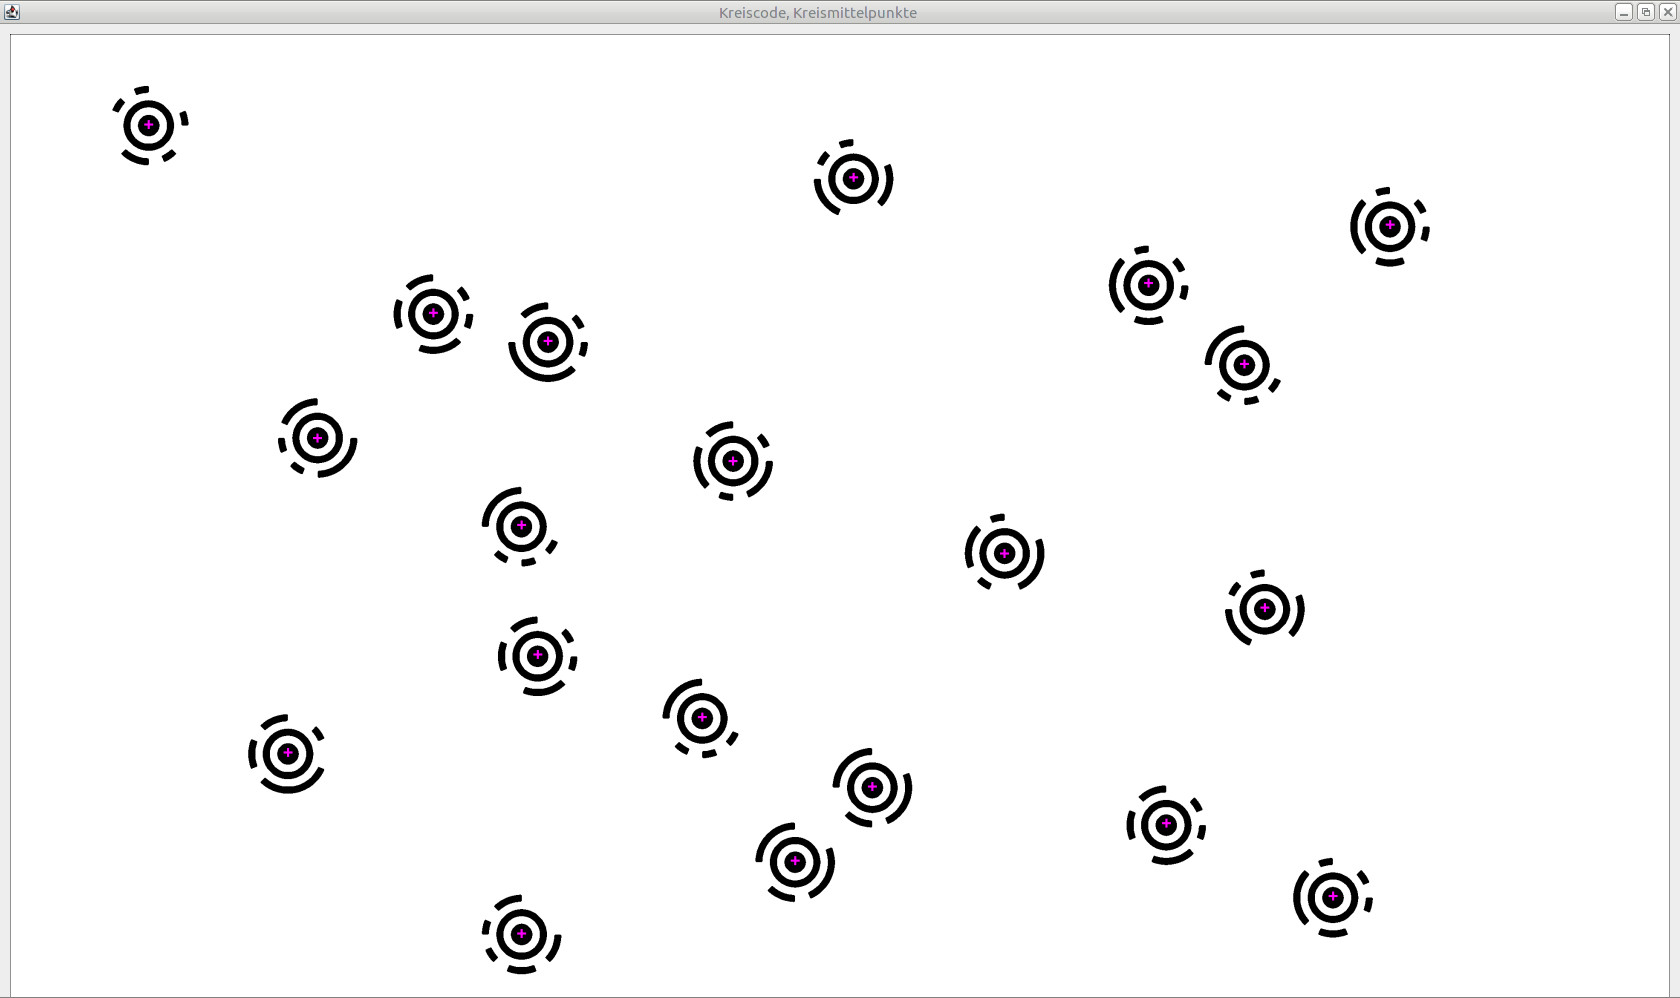
\includegraphics[width=\textwidth]{sek1bsp1}
	\caption{Beispielbild d. Aufgabenstellung}
\end{figure}
	\chapter{Dekodiermodul}
		\section{Lösungsidee}
	\begin{wrapfigure}{r}{0.35\textwidth}
		\setlength\intextsep{0pt}
		\centering
		\begin{tikzpicture}[scale=0.3]
	\fill[black!90!white] (0,0) circle [radius=1.5];
	\fill[black!90!white, even odd rule] (0,0) circle[radius=2.5] circle[radius=3.5];
	\fill[black!60!white, even odd rule] (0,0) circle[radius=4.5] circle[radius=5.5];

	\foreach \angle in {0, 22.5, 45, 67.590, 90, 112.5, 135, 157.5, 180, 202.5, 225, 247.5, 270, 292.5, 315, 337.5} 
    	\draw[thick] (0,0) -- (\angle:5.5);

	\fill[red] (0,0) circle[radius=0.2];
\end{tikzpicture}

		\caption{Geraden}
		\label{abb:spidergrafik}
		\vspace{-20pt}
	\end{wrapfigure}
	Zunächst habe ich den \task{} mit TikZ nachgezeichnet, um den genauen Aufbau durch Nachbau zu verstehen. Die 16 gleichgroßen Kreissegmente sind durch Strahlen getrennt, die im Abstand von \(22,5^{\circ}\) vom Pol (dem Mittelpunkt) aus gezeichnet werden. Der Abstand zwischen den Strahlen beträgt im Bogenmaß \(\frac{22,5\pi}{180}\).

	Für die Dekodierung steht mir aus dem Kreismittelpunkterkennungsprozess die Liste der Kreismittelpunkte zur Verfügung. Die Kreisdurchmesser entsprechen der Länge der Zusammenhangskomponenten an den Mittelpunktskoordinaten. Mit diesen Informationen kann ich dank bekannter Proportionen eines \task{}s auf die Position des äußeren Ringes, der die Informationen trägt, schließen (siehe Abb. \ref{abb:dims}). Wie in der Lösungsidee zur Kreismittelpunkterkennung festgestellt gilt \(u=\frac{1}{3}d\).

	\begin{wrapfigure}{r}{0.25\textwidth}
		\setlength\intextsep{0pt}
		\centering	
		\begin{tikzpicture}[scale=0.75]
	\clip (-1,-0.4) rectangle (6, 3);
	\fill[black!60!white, even odd rule] (0,0) circle[radius=4.5] circle[radius=5.5];

	\foreach \angle in {0, 22.5, 45, 67.590, 90, 112.5, 135, 157.5, 180, 202.5, 225, 247.5, 270, 292.5, 315, 337.5} 
    	\draw[thick] (\angle:4.5) -- (\angle:5.5);

	\filldraw[fill=green!20,draw=green!50!black] (0,0) -- (2,0) arc[start angle=0, end angle=22.5, radius=2];
	\draw[green!50!black, thick] (0,0) -- (22.5:4.5);

	\draw (2, 1.3) node {\(4,5u\)};
	\draw (2.7, 0.4) node {\(22,5^{\circ}\)};

	\draw[very thin] (-6, -6) grid (6, 6);
	\draw[thick] (-6, 0) -- (6, 0);
	\fill[red] (0,0) circle[radius=0.2];
\end{tikzpicture}
		\caption{}
		\label{abb:trigon}
	\end{wrapfigure}
	Daher kann ich mithilfe von polaren Koordinaten\footnote{\url{https://www.lernhelfer.de/schuelerlexikon/mathematik-abitur/artikel/polarkoordinatensystem}} die Strecken, die die Kreisringe in Segmente einteilen, bestimmen. Jede der Strecken ist Teil eines Strahls, der am Mittelpunkt in einem Vielfachen von \(22,5^{\circ}\) beginnt. Die eigentlichen Strecken, die auf dem äußeren Kreisring liegen, beginnen nach einem Abstand von \(4,5u\) und enden bei \(5,5u\). Die Anfangs- und Endpunkte aller Strecken lauten also:

	\begin{displaymath}
	A(k \cdot 22,5^{\circ}:4,5u) \hspace{2em} B(k \cdot 22,5^{\circ}:5,5u) \hspace{2em} k = \{\mathbb{N}_0 \hspace{0.3em}|\hspace{0.3em} 0 \le x \le 15\}
	\end{displaymath}

	Da der Strahl zusammen mit der Achse, von der aus der Winkel gemessen wird, ein rechtwinkliges Dreieck bildet (s. Abb \ref{abb:trigon}), könnenen wir die Punkte der Strecke in kartesischen Koordinaten berechnen. Ich habe das Koordinatensystem in der Einheit \(u\) gezeichnet. Bitte stellen sie Ihren Taschenrechner vorher auf "`rad"' ein!

	\begin{gather}
	k = \{\mathbb{N}_0 \hspace{0.3em}|\hspace{0.3em} 0 \le x \le 15\} \\
	\begin{split}
	x_{innen} &= cos(k \cdot \frac{22,5\pi}{180}) \cdot 4,5u \\
	y_{innen} &= sin(k \cdot \frac{22,5\pi}{180}) \cdot 4,5u
	\end{split}
	\hspace{5em}
	\begin{split}
	x_{aussen} &= cos(k \cdot \frac{22,5\pi}{180}) \cdot 5,5u \\
	y_{aussen} &= sin(k \cdot \frac{22,5\pi}{180}) \cdot 5,5u
	\end{split}
	\end{gather}

	\begin{figure}[!ht]
		\begin{subfigure}[b]{0.5\textwidth}
			\centering	
			\begin{tikzpicture}[scale=0.5]
	\fill[black!90!white] (0,0) circle [radius=1.5];
	\fill[black!90!white, even odd rule] (0,0) circle[radius=2.5] circle[radius=3.5];
	\fill[black!60!white, even odd rule] (0,0) circle[radius=4.5] circle[radius=5.5];
	
	\foreach \angle in {0, 22.5, 45, 67.590, 90, 112.5, 135, 157.5, 180, 202.5, 225, 247.5, 270, 292.5, 315, 337.5} 
    		\fill[red] (\angle:4.5) circle [radius=0.1] (\angle:5.5) circle [radius=0.1]; 

	\draw[very thin] (-6, -6) grid (6, 6);
	\fill[red] (0,0) circle[radius=0.2];
\end{tikzpicture}
			\caption{Einteilende Punkte}
		\end{subfigure}
		\begin{subfigure}[b]{0.5\textwidth}
			\centering	
			\begin{tikzpicture}[scale=0.5]
	\fill[black!90!white] (0,0) circle [radius=1.5];
	\fill[black!90!white, even odd rule] (0,0) circle[radius=2.5] circle[radius=3.5];
	\fill[black!60!white, even odd rule] (0,0) circle[radius=4.5] circle[radius=5.5];

	\foreach \angle in {0, 22.5, 45, 67.590, 90, 112.5, 135, 157.5, 180, 202.5, 225, 247.5, 270, 292.5, 315, 337.5} 
    	\draw[blue, thick] (\angle:4.5) -- (\angle:5.5) -- (\angle+22.5:5.5) -- (\angle+22.5:4.5) -- cycle;

    	
	\draw[very thin] (-6, -6) grid (6, 6);
	\fill[red] (0,0) circle[radius=0.2];
\end{tikzpicture}
			\caption{Trapeze}
		\end{subfigure}
	\end{figure}

	Wenn wir nun alle benachbarten Koordinaten verbinden, erhalten wir 16 Trapeze, die fast den Kreissegmenten entsprechen. Da die Abweichung zwischen dem jeweiligen Trapez und dem jeweiligen Kreissegment sehr gering ist, kann aus den Pixeln im Trapez auf die Farbe des Ringsegmentes geschlossen werden. Da das ganze Ringsegment entweder ganz weiß oder ganz schwarz ist, entspricht die vorherrschende Farbe im Trapez der Farbe des Kreissegmentes.
\section{Umsetzung}
	Die vorherrschende Farbe kann mit einer Flood-Fill über die Trapezfläche ausgezählt werden. Hierfür benötigen wir zum einen für jedes der 16 Trapeze einen Startpunkt. Zum anderen muss für die Flood-Fill die Linien des Trapezes bestimmt werden, sodass die Flut die Trapezfläche nicht verlässt.

	Für die Bestimmung der Startpunkte nummerieren ich die Segmente von 0 bis 15. Wenn man nun die x- und y-Koordinaten aller anliegende Punkte arithmetisch mittelt, erhält man den Mittelpunkt des Trapezes. Die Formel für die Koordinaten eines \textit{n}ten-Trapezes eines Kreis-Codes mit dem Mittelpunkt \(x_0 . y_0\) lautet:
	\begin{gather}
	\begin{split}
		x_1 &= cos(n \cdot \frac{22,5\pi}{180}) \cdot 5,5u + x_0\\
		y_1 &= sin(n \cdot \frac{22,5\pi}{180}) \cdot 5,5u + y_0\\ \vspace{2em}
		x_2 &= cos(n \cdot \frac{22,5\pi}{180}) \cdot 4,5u + x_0\\
		y_2 &= sin(n \cdot \frac{22,5\pi}{180}) \cdot 4,5u + y_0
	\end{split}
	\hspace{5em}
	\begin{split}
		x_3 &= cos((n+1) \cdot \frac{22,5\pi}{180}) \cdot 5,5u + x_0\\
		y_3 &= sin((n+1) \cdot \frac{22,5\pi}{180}) \cdot 5,5u + y_0 \\ \vspace{2em}
		x_4 &= cos((n+1) \cdot \frac{22,5\pi}{180}) \cdot 4,5u + x_0\\
		y_4 &= sin((n+1) \cdot \frac{22,5\pi}{180}) \cdot 4,5u + y_0
	\end{split} \label{eq:nKoords}
	\end{gather}
	\begin{equation}
	x = \frac{(x_1+x_2+x_3+x_4)}{4} \hspace{4em} y = \frac{(y_1+y_2+y_3+y_4)}{4}
	\end{equation}
	Abschließend müssen die x- und y-Werte noch gerundet werden, da im gerasterten Bild nur ganzzahlige Pixel adressierbar sind.
	Zur Überprüfung habe ich ein kleines CPP-Programm geschrieben, welches die Formel für \(n = 0\hspace{2pt}..\hspace{2pt}15 \) durchrechnet und entstprechende TikZ-Anweisungen ausgibt (Quellcode: mittelpunkte.cpp). Obwohl sehr ungenau auf Vielfache von \(u\) gerundet wurde, liegen alle Punkte in ihrem jeweiligen Segment.
	\begin{figure}[!ht]
		\centering
		\begin{tikzpicture}[scale=0.5]
	\fill[black!90!white] (0,0) circle [radius=1.5];
	\fill[black!90!white, even odd rule] (0,0) circle[radius=2.5] circle[radius=3.5];
	\fill[black!60!white, even odd rule] (0,0) circle[radius=4.5] circle[radius=5.5];
	
	\fill[red] (5,1) circle [radius=0.1]; 
	\fill[red] (4,3) circle [radius=0.1]; 
	\fill[red] (3,4) circle [radius=0.1]; 
	\fill[red] (1,5) circle [radius=0.1]; 
	\fill[red] (-1,5) circle [radius=0.1]; 
	\fill[red] (-3,4) circle [radius=0.1]; 
	\fill[red] (-4,3) circle [radius=0.1]; 
	\fill[red] (-5,1) circle [radius=0.1]; 
	\fill[red] (-5,-1) circle [radius=0.1]; 
	\fill[red] (-4,-3) circle [radius=0.1]; 
	\fill[red] (-3,-4) circle [radius=0.1]; 
	\fill[red] (-1,-5) circle [radius=0.1]; 
	\fill[red] (1,-5) circle [radius=0.1]; 
	\fill[red] (3,-4) circle [radius=0.1]; 
	\fill[red] (4,-3) circle [radius=0.1]; 
	\fill[red] (5,-1) circle [radius=0.1];  

	\foreach \angle in {0, 22.5, 45, 67.590, 90, 112.5, 135, 157.5, 180, 202.5, 225, 247.5, 270, 292.5, 315, 337.5} 
	\draw[blue, thick] (\angle:4.5) -- (\angle:5.5) -- (\angle+22.5:5.5) -- (\angle+22.5:4.5) -- cycle;

	\draw[very thin] (-6, -6) grid (6, 6);
	\fill[red] (0,0) circle[radius=0.2];
\end{tikzpicture}
		\caption{Mittelpunkte}
	\end{figure}

	Um die Flood-Fill durchführen zu können, müssen nun die Grenzen der Trapeze bestimmt werden. 

	Alle Trapeze im Kreisring bestehen aus 16 Strecken, die den Kreisring einteilen sowie 16 obere- wie untere Strecken. Daher muss ich in die Grafiken für jedes \textit{n} folgende Punkte aus Gleichung \eqref{eq:nKoords} verbinden.:
	
	\begin{equation}
		\overline{P_1P_2} \hspace{3em}
		\overline{P_2P_4} \hspace{3em}
		\overline{P_1P_3} \hspace{3em}
	\end{equation}

	Wenn ich diese Strecken nun in eine weiteres Array einzeichne, erhalte ich Grenzen für die Flut von den soeben berechneten Mittelpunkten aus. Arrays entsprechen einer Rastergrafik. Das Einzeichen von geometrischen Formen in Rastergrafiken wird in der Literatur \textit{rastern} genannt. Meine Anforderungen an den Rasterisierungsalgorithmus lauten:
	\begin{itemize}
		\item Möglichst geringe Laufzeit
		\item Lückenlosigkeit, d.h die Linie muss ein durchgehender Pfad durch die Rastergrafik sein
	\end{itemize}
	Ausdrücklich nicht benötigt wird eine besonders schöne oder besonders genaue Rasterisierung, es muss nur ein möglichst großer Teil des Trapezes innerhalb der Linien liegen. Die gerasterten Linien werden dem Nutzer außerhalb von Debug-Funktionen niemals angezeigt.

	Ich habe mich über Rasteralgorithmen in einer Zusammenfassung eines Proseminars an der TU Dresden\footnote{\url{https://www.inf.tu-dresden.de/content/institutes/smt/cg/teaching/seminars/ProseminarSS08/skurfuerst/latex-doc.pdf}} informiert. Das PDF habe ich der Einsendung beigefügt.
	
	Der auf den Seiten 3 bis 5 und in einem YouTube-Talk\footnote{\url{https://youtu.be/zytBpLlSHms}} vorgestellte Bresenham-Algorithmus trifft mein Anforderungsprofil genau: Er zeichnet in Linearzeit eine 1px breite Linie zwischen zwei Punkten. Da der Algorithmus ausschließlich mit Ganzzahlen arbeitet, müssen alle Koordinaten vor Eingabe in den Algorithmus gerundet werden.
\section{Beispiele}

	\chapter{Erkennung von Fotos}
		\section{Lösungsidee}
\begin{wrapfigure}{r}{0.45\textwidth}
		\setlength\intextsep{0pt}
		\centering	
		\includegraphics[width=0.4\textwidth]{Grafiken/sek3abb1}
		\caption{Verbesserte Bilderkennung}
		\label{abb:transform}
	\end{wrapfigure}
Die in Kapitel 1 vorgestellte Einleseprozedur wird den Anforderungen für die Erkennung eines Fotos oder eines Scans nicht gerecht. Bei schankender Ausleuchtung des Bildes lässt sich kein geeigneter Schwellwert bestimmen. Stattdessen wende ich verschiedene Algorithmen des maschinellen Sehens an, um ein möglichst ideales Bild aus dem Eingabebild zu extrahieren.

Ich extrahiere zunächst alle Kanten des Bildes. Kanten sind Stellen, an denen sich die Farbwerte eines Pixels schlagartig ändern. Den Kantextraktionsalgorithmus implementiere ich hierbei so, dass die Kante eine lückenlose Linie darstellt.

Mit diesen Kanten habe ich das Bild segmentiert. Anschließend fülle ich jedes Segment komplett schwarz (1) oder weiß (0).
Der Bestimmung der Farbe der Füllung lege ich folgende Annahme zu Grunde:

Der Hintergrund des Bildes ist komplett weiß. Alle an den Hintergrund angrenzenden Segmente sind schwarz, schließlich fand dort eine schlagartige Farbänderung zum Hintergrund statt. Die Felder, die an diese Segmente angrenzen sind weiß, da sich die Farbe widerum schlagartig geändert hat. Dieses Muster setze ich fort, bis die Farben aller Segmente bestimmt sind.

Die drei Schritte der Bildprozessierung sind in Abbildung \ref{abb:transform} dargestellt.

Vorteil dieser Vorhergehensweise über ein Schwellwertverfahren ist, dass jeder ähnlich gefärbte Bereich die selbe Farbe erhält. Ein zusammen gehörender Bereich enthält keinerlei Lücken. Dies ist für den Kreismittelpunkterkennungsalgorithmus essenziell, da sonst die Radiusbestimmung fehlschlägt.
 
\section{Umsetzung}
\subsection{Graustufenbild}
In einem ersten Schritt bestimme ich aus dem farbigen Bild ein Graustufenbild. Dies erfolgt mit einer gewichteten Mittelung aus den Intensitätswerten der drei Primärfarbkanäle. Laut der Norm CIE 1931\footnote{\url{en.wikipedia.org/wiki/Grayscale}} ist der Grauwert mit folgender Formel zu bestimmen:

\begin{equation}
Y = 0,2126R+0,7152G+0,0722G
\end{equation}

\subsection{Canny-Edge-Detector}
\subsubsection{Weichzeichnung}
Darauf filtere ich vor der eigentlichen Kantenerkennung grobe Außreißer aus dem Bild heraus. Hierfür wende ich einen Gaußschen Weichzeicher an. Ein solcher Weichzeichner funktioniert, indem für jedes Pixel ein gewichteter Mittelwert aus seinem eigenen Grauwert und den Grauwerten seiner Umgebung bestimmt wird. Der Gewichtung wird die Gaußsche Normalverteilung zugrunde gelegt. Ich habe mich für ein Sigma von 3 entschieden. Mit dieser Kurve werden große Ausreißer entfernt, der Kantenverlauf bleibt jedoch erhalten. Aus dieser Kurve lässt sich folgende Matrix extrahieren\footnote{\url{http://dev.theomader.com/gaussian-kernel-calculator/}}:
\begin{equation}
	\begin{bmatrix}
	0,031827&0,037541&0,039665&0,037541&0,031827 \\
	0,037541&0,044281&0,046787&0,044281&0,037541 \\
	0,039665&0,046787&0,049434&0,046787&0,039665 \\
	0,037541&0,044281&0,046787&0,044281&0,037541 \\
	0,031827&0,037541&0,039665&0,037541&0,031827 \\
	\end{bmatrix}
\end{equation}
Jeder Pixel wird mit dem mittleren Wert multipliziert. Die umliegenden Pixel werden mit ihren Pendants in der Matrix multipliziert. Die Summe aus allen Produkten entspricht dem neuen Wert des Pixels.

Allerdings kann die Gaußsche Weichzeichnung auch in einen horizontalen und vertikalen Bestandteil aufgeteilt werden. Bei dieser Aufteilung erhält man folgende Matrix:
\begin{equation}
	\begin{bmatrix}
	0,1784&0,210431&0,222338&0,210431&0,1784
	\end{bmatrix}
\end{equation}
Man kann mit dieser Matrix das gleiche Ergebnis erzielen, indem man sie zunächst in horizontale und anschließend in vertikale Richtung anwendet. Diese Vorhergehensweise hat eine bessere Laufzeit, da für die Glättung eines Pixels nicht \(4^2\) sondern nur \(2\times 4\) Pixel betrachtet werden müssen.

\subsubsection{Sobel-Operator}
Anschließend wende ich auf das nun geglättete Bild den Sobel-Operator an. Dieser Operator entspricht der 1. Ableitung über die Helligkeitskurve des Bildes. Der Operator wird mithilfe von \textit{Convolution} über das gesamte Bild berechnet. Convolution ist das aus dem Gauß-Wiechzechner bekannte Prinzip, dass auf jedes Pixel eine Matrix angewandt wird. Der Sobel-Operator funktioniert mit zwei Convulution-Durchläufen mit folgenden Matrizen:
\begin{gather}
	\begin{split}
		\begin{bmatrix}
			-1,0&-2,0&-1,0\\
			0,0&0,0&0,0\\
			1,0&2,0&1,0\\
		\end{bmatrix}
	\end{split}
	\hspace{5em}
	\begin{split}
		\begin{bmatrix}
			-1,0&0,0&1,0\\
			-2,0&0,0&2,0\\
			-1,0&0,0&1,0\\
		\end{bmatrix}
	\end{split}
\end{gather}

Diese Matrizen entsprechen der Ableitung in vertikale und horizontale Richtung, da die jeweils angrenzenden Felder voneinander subtrahiert werden. Wenn die umliegenden Pixel den gleichen Intensitätstwert haben ist das Ergebnis des Sobel-Operators 0. Bei Intensitätsunterschieden verändert sich das Ergebnis des Operators entsprechend.
Da allerdings eine Ableitung und nicht zwei Ableitungen gwünscht sind, müsse beide Ableitungswerte eines Pixels vereinigt werden. Dies gelingt mit dem Satz des Pythogoras. Die Ausschläge der Ableitungen in x- und y-Richtungen entsprechen den Kateten. Ein kombinierter Wert aus beiden Ableitungen ist daher aus der Länge der Hypothenuse gegeben.

\subsubsection{Non-Maximum-Supression (Nichtmaximumsunterdrückung)}
Allerdings sind die Bereiche mit einem Ableitungswert über 0 mehrere Pixel breit. Schlißlich sind die Kanten im Bild nicht wirklich abrupt, sondern verlaufen über mehrere Pixel. Allerdings kann mit der Tangensfunktion der Winkel der Kante ermittelt werden:
\begin{equation}
	tan(\alpha) = \frac{G_y}{G_x}
\end{equation}

Mit diesem Winkel können die Pixel bestimmt werden, die an der gleichen Kante liegen. Wenn der Pixel nicht das Maximum an der Kante ist kann sein Ableitungswert auf 0 gesetzt werden (Der Pixel wird in der Ausgabegrafik unterdrückt). Schließlich gibt es entlang der Kante einen größeren Ausschlag.  

Wenn der Winkel beispielsweise 0 beträgt, verläuft die Katen in horizontale Richtung. Dann wird der Ableitungswert des Pixels mit seinem nördlichen und südlichen Nachbarn verglichen. Nur wenn der Ableitungswert das Maximum von diesen Pixeln darstellt, ist er Teil der 1px breiten Kante.

\subsubsection{Binärisierung mit Hysterese}
Zur Binärisierung des Ergebnisses der Sobel-Operators wende ich eine Technik namens \textit{Hysterese} an. Bei einer Hysterese wird zunächst mit einem hohen Schwellwert das Bild binärisiert. Das heißt im Kontext  meiner Implementierung, dass alle Pixel mit ein Ableitungswert höher 50 im Ausgabebild schwarz gefärbt werden.

Da aber möglicherweise eine Kante auch aus weniger stark abgesetzten Pixeln besteht, akzeptiert die Hysterese für an erkannte Aktenpunkte anliegende Punkte einen niedrigeren Schwellwert.

Dies ist als Stack implemementiert. Jedes im ersten ersten Erkennungsschritt erkannte Pixel wird auf diesen Stack gelegt. Nach Abschlussd es ersten Erkennungsschrittes werden alle Pixel, die an ein Pixel aus dem Stack angrenzen, noch nicht markeirt wurden und über dem verringerten Schwellwert von 12,5 liegen, schwarz markiert. Diese Pixel werden widerum auf den Stack gelegt, sodass die Kante mti dem verrignerten Schwellwert verfolgt wird. 

\subsubsection{Erosion}
Aufgrund der Non-Maximum-Supression sind kleine Lücken in der Grafik entstanden. Diese Verhindern eine sinnvolle Ausführung der nachfolgenden Flood-Fill. Daher erdodiere ich das Ergebnis der Hysterese. Erodierung bedeutet, dass jedes Pixel, dass mehr als einen schwarzen Nachbarn hat, geschwärzt wird.
Damit verdicke ich wieder die Linie, jedoch ist sie weiterhin weitaus exakter, als sie es ohne Non-Maximum-Supression wäre. 

\subsection{Einfärben des Bildes}
Der Canny-Detektor gibt ein Bild aus den Kanten aus. Die weiteren Berechnungsschritte benötigen jedoch ein Bild, in dem der Kreis, der Kreisring und die Segmente komplett schwarz eingefärbt. Unter Ausnutzung der Annahme aus der Lösungsidee habe ich einen Algorithmus formuliert. Dieser nimmt als Eingabe das Ergebnis des Canny-Eckenerkennungsprozesses und hat als Ausgabe ein Binärbild als boolesches 2D-Array. Damit ist die Ausgabe der neuen Bidleinleseprozedur identisch zu der Ausgabe der ersten Einleseprozedur aus Kapitel 1. 
Vom Pixel(0|0) ausgehend werden alle direkt erreichbaren weißen Pixel mithilfe einer Flood-Fill im Ausgabebild als weiß abgespeichert, da diese den Hintergrund darstellen.
Anschließend weden alle schwarzen Pixel, die an den Hintergrund angrenzen, als schwarz markiert. Diese Pixel stellen die Kante zum Vordergrundbereich dar. Da sie nur die Kante des Vordergrundbereiches sind, werden alle an diese Pixel angrenzenden weißen Pixel im Ausgabebild als Schwarz markiert. Schließlich befinden wir uns weiterhin im Vordergrund. Diese Prozedur wird abwechselnd zur Bestimmung von Vorder- und Hintergrundbereichen eingesetzt.
\section{Beispiele}

\end{document}
